The aim of this coursework is to implement and train a fully connected neural net to classifiy emotions using images of faces.
There are 7 emotions, namely: anger, disgust, fear, happiness, sadness, surprise and neutral.
This report discusses our approach and findings.
First, we discuss the theory behind neural nets.
Next, we explain how we tuned our neural net's hyperparameters
and provide an analysis of our model using metrics such as confusion matrices or recall rates.
We conclude with an exploration of neural net state of the art explorat

But first, what is neural network?
Neural networks aim to mimic the biological neural network present in the human brain.
Let us begin by explaining the concept of a neuron.

\begin{center}
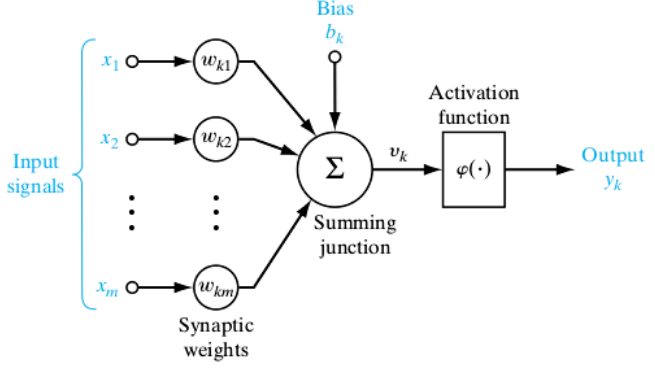
\includegraphics[scale = 0.35]{src/diagrams/neuron_diagram.png}
\end{center}

A neuron takes in several inputs and produces a single output, as represented in the picture above.
The neuron sums all inputs weighted by their respective weights,
adds a bias and then inputs this into an activate function to produce a single output.


\begin{center}
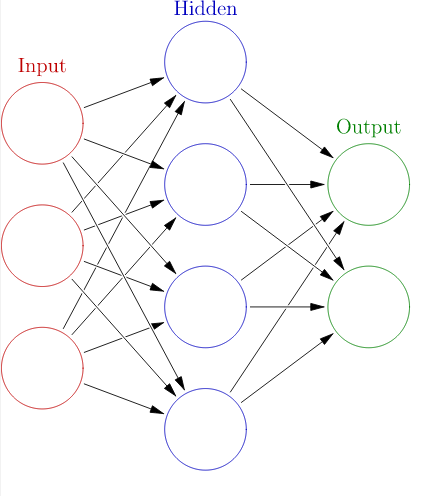
\includegraphics[scale = 0.35]{src/diagrams/neural_net_diagram.png}
\end{center}

A neural network is is composed of layers of neurons,
such that each neuron's output is an input to all of the next layer's neurons.
The diagram below, shows three different types of layers.
The input layers contains a neuron for each data input's elements.
These neurons simply output the data point's element they are given.
The hidden layer's neurons have a respective weight for each of the inputs connected to them,
and produces a single output as described earlier.
The output layer's neurons also have weights for each input,

